\documentclass{article}

\usepackage[top=2in, bottom=1.5in, left=1in, right=1in]{geometry}
\usepackage{fancyhdr} 		% page header
\usepackage{amsmath}
\usepackage{amssymb}
\usepackage{float}
\usepackage{graphicx}
\usepackage{url}
\usepackage{tikz}
\usetikzlibrary{shapes.geometric}
\usetikzlibrary{positioning}
\usepackage{hyperref}

\pagestyle{fancy} 
\fancyhf{}
\fancyhead[L]{CS 540}
\fancyhead[R]{Fall 2018}

\def\x{\mathbf{x}}
\def\y{\mathbf{y}}
\def\w{\mathbf{w}}
\def\p{\mathbf{p}}

\begin{document}


\begin{center}
{\bf \large CS 540-1: Introduction to Artificial Intelligence

Homework Assignment \# 5

\vspace{0.5cm}

Assigned:  10/4 

Due:  10/11 before class} 
\end{center}

\vspace{1cm}

\begin{center}
{\bf \Large Hand in your homework:}
\end{center}

This homework includes only written questions. 
Please submit a single \textbf{hw5.pdf} file -- we recommend latex, but you can use anything that can render nice math.
Please typeset your homework, do not submit handwritten+scan answers.
Go to UW Canvas, choose your CS540-1 course, choose Assignment, click on Homework 5: this is where you submit your files. 

\section*{Question 1: Game Tree Search [50 points]}
Consider the game tree below. 
Let $\Delta$ and $\nabla$ nodes represent nodes belonging to the maximizing and minimizing player respectively.

\begin{figure}[ht]
\centering
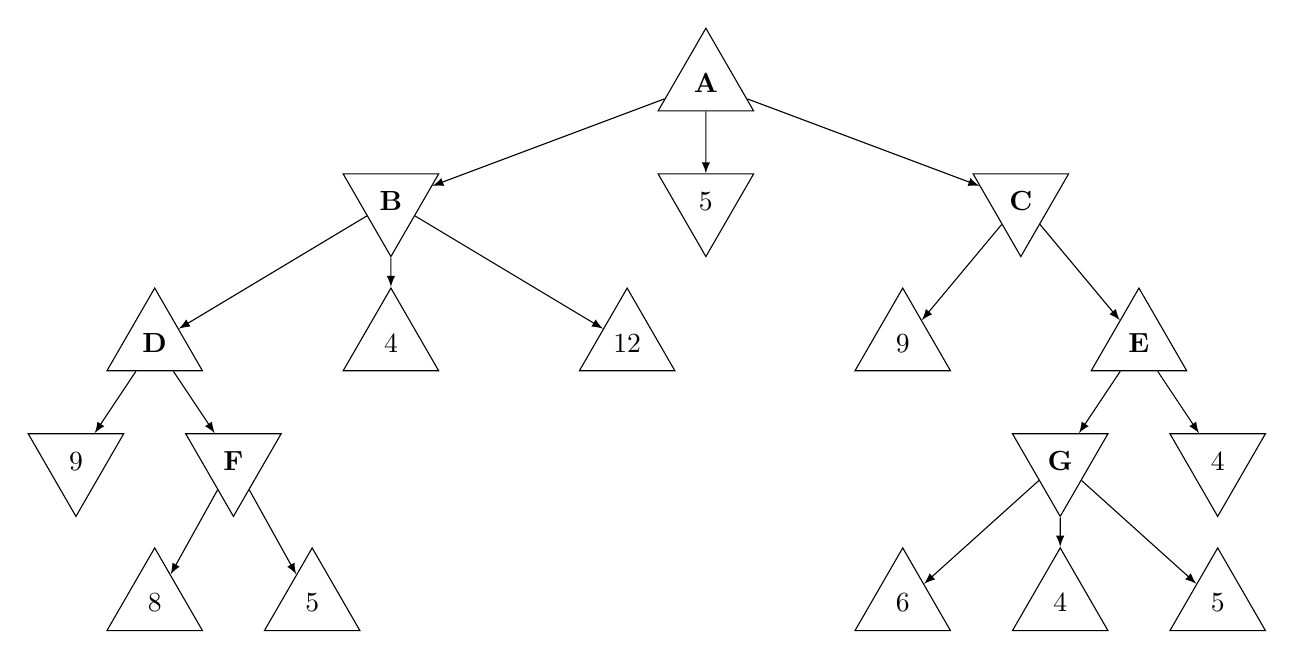
\begin{tikzpicture}[edge from parent/.style={draw,-latex},
    triangle/.style = {regular polygon, regular polygon sides=3, minimum size=1.4cm, inner sep=0pt},
    border rotated/.style = {shape border rotate=180},
    level 1/.style={sibling distance=4cm, level distance=1.5cm},
    level 2/.style={sibling distance=3cm, level distance=1.8cm},
    level 3/.style={sibling distance=2cm, level distance=1.5cm},
    level 4/.style={sibling distance=2cm, level distance=1.8cm}]
    \node [triangle,draw]{\textbf{A}}
        child {node [triangle,border rotated,draw]{\textbf{B}}
            child {node [triangle,draw]{\textbf{D}}
                child {node [triangle,border rotated,draw]{9}}
                child {node [triangle,border rotated,draw]{\textbf{F}}
                	child {node [triangle,draw]{8}}
                	child {node [triangle,draw]{5}}
                }
            }
            child {node [triangle,draw]{4}}
            child {node [triangle,draw]{12}}
        }
        child {node [triangle,border rotated,draw]{5}}
        child {node [triangle,border rotated,draw]{\textbf{C}}
            child {node [triangle,draw]{9}}
            child {node [triangle,draw]{\textbf{E}}
                child {node [triangle,border rotated,draw]{\textbf{G}}
                	child {node [triangle,draw]{6}}
                	child {node [triangle,draw]{4}}
                	child {node [triangle,draw]{5}}
                }
                child {node [triangle,border rotated,draw]{4}}
                }
        };
\end{tikzpicture}
\end{figure}

\begin{enumerate}

\item (20 points) 
    Use the minimax algorithm to 
    \begin{enumerate}
	\item compute the game theoretical value at EACH node; 
	\item list the set of optimal moves, namely ones that achieve the game theoretical value at the node, for the corresponding player at EACH node.
    \end{enumerate}

\item (20 points)
	Use alpha-beta pruning to compute the Minimax value at each node for the
	same game tree. Assume that nodes 
	are visited from left to right. Show your alpha and beta values at EACH node 
	after the final time it is visited. Also clearly indicate the subtrees that are pruned (if any).

\item (10 points)
	Does there exist a game tree where minimax and alpha-beta pruning algorithms have the potential to produce 
	different moves? Justify your answer.


\end{enumerate}


\section*{Question 2: Probability [50 points]}
\begin{enumerate}

\item (10 points) Consider the two events:

\begin{itemize}
	\item Roll two fair dice with a total of seven.
	\item Roll three fair dice with a total of seven.
\end{itemize}

Which of these is more likely to happen? Justify your answer by computing the probability of each event.

\item (10 points) John and Robert play a game with a pile of 52 cards. The player who gets the Ace of Hearts wins. John and Robert pick up 2 cards each. John shows his cards to Robert first, but John’s cards does not contain the Heart Ace. What is the probability of Robert winning? 

\item (10 points) 1 out of 10000 clover leaves has four leaflets.  Assuming clover leaves are picked randomly and independently.  How many clover leaves does one need to inspect in order to find a four-leaf clover with probability at least 0.9?

\item (10 points) There are three cards in an opaque box. The first card is painted black on both sides, the second card is painted red on both sides, and the third card has one side black and one side red. One picks a card randomly and observes one side of this card is black (without seeing the other side). What is the probability that the other side is red?

\item (10 points)  Suppose that the probability of the word ‘lottery’ appearing in a spam email is 42\%, and the probability of it appearing in a non-spam email is 5\%. If every email received has equal probability of being spam or not spam, what is the probability that an email is spam given it contains the word ‘lottery’?


\end{enumerate}






\end{document}
